\section{Activity Structure}
\label{implementation:activity_structure}
\begin{figure}[h!]
	\centering
	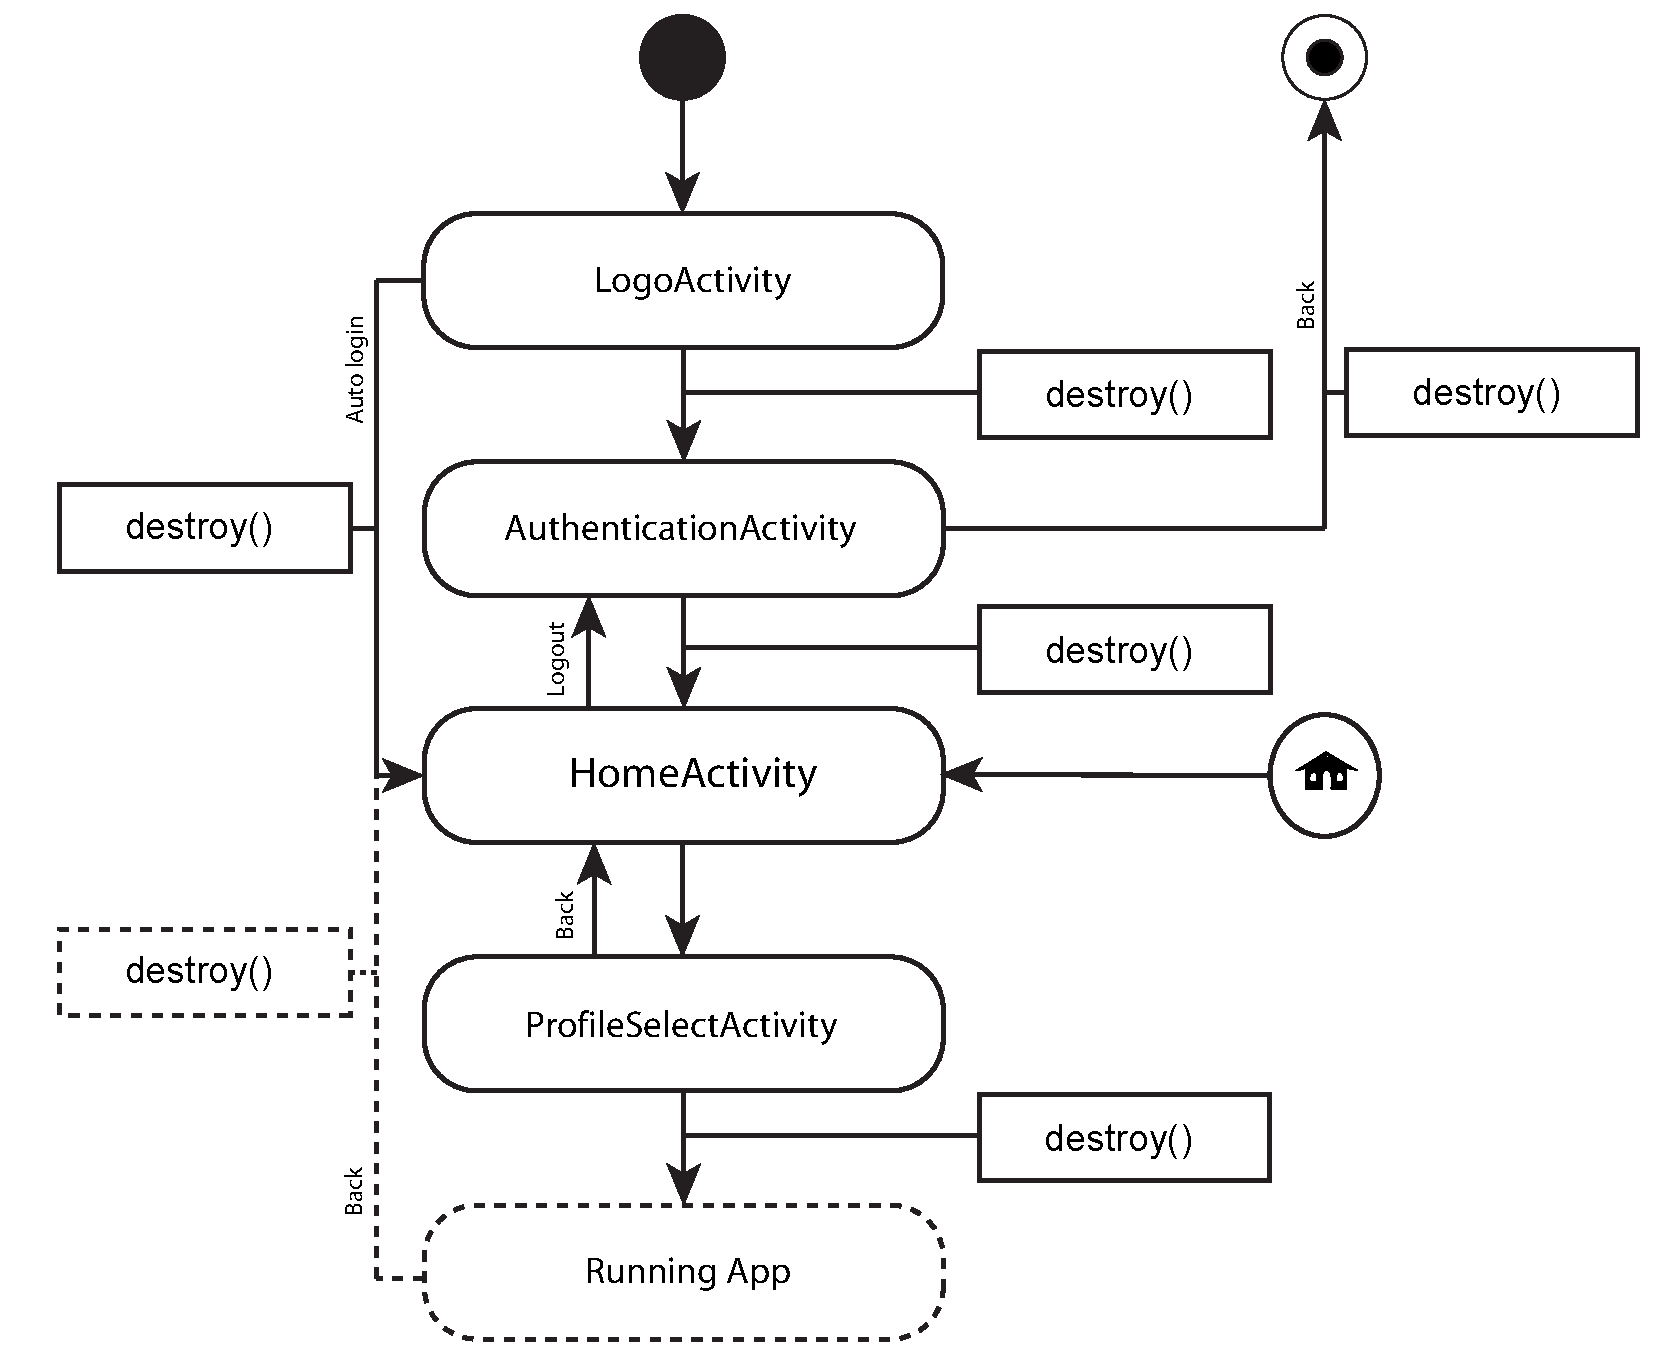
\includegraphics[width=1\textwidth]{gfx/activityDiagram.pdf}
	\caption{Activity diagram of the launcher}
	\label{fig:activity_diagram}
\end{figure}
\autoref{fig:activity_diagram} shows the activity structure of the \giraf[] launcher. Every path with a \verb+destroy()+ box on it gets the activity starting the path destroyed. Everytime the user is outside the launcher and hits the home button they will end up in the \activity{HomeActivity}, if the \giraf[] launcher is set to the default launcher.
The dotted line from Running App to \activity{HomeAcitivity} symbolizes that the app it self can handle the back press but if there is not done something active to handle this action the default action is to return to the \activity{HomeAcitivity} and destroy the app from the backstack.

When the launcher is started the user is presented with the \activity{LogoActivity} from where they will be redirected to the \activity{AuthenticationActivity} to preform the login. In this process the \activity{LogoActivity} gets destroyed from the backstack.
It is possible for the user to easily quit in the \activity{AuthenticationActivity} if they do not have their QR code at hand. If the user makes an valid login they will be send to the \activity{HomeActivity}. As the main activity it is possible to come from here and to \activity{AuthenticationActivity} or \activity{ProfileSelectActivity}. If the user clicks on an app they will be presented with the \activity{ProfileSelectActivity} and have to choose a child before they can start the app.


\todo{REFACTOR GIRAF COMPONENTS!}